\NeedsTeXFormat{LaTeX2e}[2005/12/01]
%%    2010/04/06 v1.0 Vorlage Master-Forschungspraktikum Versuchsauswertung
%%    based on the 2009/10/14 v0.1 GAUBM template by Prof Pruschke

\documentclass[twoside,        %% zweiseitiges Layout
               BCOR12mm,       %% Bindekorrektur 12 mm
% please comment out if report is in English
               english,ngerman, %% Dokumentspr. Deutsch, Alternativspr. Englisch
% please remove comment if report is in English 
%               ngerman,english, %% Dokumentspr. Englisch, Alternativspr. Deutsch
               fleqn,headsepline=false,footsepline=false
              ]{Vorlage/MFPREPORT}

%% Pakete und Definitionen ausgelagert
\input{Vorlage/packages}
\input{Vorlage/layout}

%% einbinden einiger nützlicher Befehle
\input{Vorlage/shortcuts}

%Zur Formatierung in der Matheumgebung
\renewcommand{\t}{\ensuremath{\rm\tiny}} % Tiefgestellter Text in der Matheumgebung wird schoener mit: $\Phi_{\t{Text}}$
\renewcommand{\d}{\ensuremath{\mathrm{d}}} % Die totale Ableitung ist stets aufrecht zu setzen: \d
\newcommand{\diff}[3][]{\ensuremath{\frac{\d^{#1}#2}{\d#3^{#1}}}} % einfache Ableitung nach x: $\ddx{\Phi}$
\newcommand{\pdiff}[3][]{\ensuremath{\frac{\partial^{#1}#2}{\partial#3^{#1}}}} % wie gesprochen, eine partielle Ableitung: \del
\newcommand{\aeqiv}{\ensuremath{\qquad \Longleftrightarrow \qquad}} % Eine Aequivalenz
\newcommand{\folgt}{\ensuremath{\qquad \Longrightarrow \qquad}} % Ein Folgepfeil mit Abstaenden
\newcommand{\corresponds}{\ensuremath{\mathrel{\widehat{=}}}} % Befehl für "Entspricht"-Zeichen
\newcommand{\mi}[1]{\ensuremath{\mathit{#1}}} % italics für griechische Buchstaben in Matheumgebung

%Um nicht so viel schreiben zu müssen...
\newcommand{\bs}[1]{\boldsymbol{#1}}
\newcommand{\ol}[1]{\overline{#1}}
\newcommand{\wtilde}[1]{\widetilde{#1}}
\newcommand{\mrm}[1]{\mathrm{#1}}
\newcommand{\mbf}[1]{\mathbf{#1}}
\newcommand{\mbb}[1]{\mathbb{#1}}
\newcommand{\mcal}[1]{\mathcal{#1}}
\newcommand{\mfrak}[1]{\mathfrak{#1}}

%Abkürzungen
\newcommand{\zB}{z.\,B.\ }
\newcommand{\bzw}{b.\,z.\, w.\ }
\newcommand{\Dh}{d.\,h.\ }
\newcommand{\Gl}{Gl.\ }
\newcommand{\Abb}{Abb.\ }
\newcommand{\Tab}{Tab.\ }


\begin{document}
\LabratoryName{FM.ULP}{Spatial and Temporal Distortion of Ultrashort Light Pulses}
\ProtocolAuthor{Eric}{Bertok}{eric.bertok@stud.uni-goettingen.de}
\Assistant{Dr. Sabine}{Steil}
\ResearchFocus{Festkörper- und Materialphysik (M.phy.403)}
% In der naechsten Version beruecksichtigt
%\Collaborator{Vorname}{Nachname}{email}
\ConductedOn{22}{11}{2017}
\date{\today}
% eines von beiden
\CopyNotWanted
%\CopyWanted

\pagenumbering{roman}
\maketitle

%\begin{otherlanguage}{english}
%\end{otherlanguage}

\tableofcontents

\clearpage
\pagenumbering{arabic}

\section{Einleitung}
\label{sec:einleitung}
\section{Theorie}
\label{sec:theorie}
\subsection{Grundlagen}
Zur Beschreibung Ultrakurzer Laserpulse verwendet man einen semiklassischen
Ansatz, bei dem die Maxwell-Gleichungen für eine makroskopische Polarisation
gelöst wird. Im Folgenden wird das Vektorfeld des elektrischen Feldes $\vec E$
durch einen Skalar $E$ genähert [Diels]. Hiermit wird eine für das Experiment
relevante Polarisationsrichtung beachtet. Im Allgemeinen sind auch Effekte
möglich, bei denen verschiedene Polarisationsrichtungen miteinander koppeln,
was eine genauere Betrachtung erfordert.
Ausgehend von dem elektrischen Feld $E(t)$ definiert man mithilfe der Fourier
Transformation das komplexe Spektrum
$\tilde{E}(\omega)=\mathcal{F}[E(t)]=\int_\mathbb{R}E(t)e^{-i\omega t}\d t
\label{eq:FT}$.
Die Rücktransformation ergibt sich zu $E(t)=\mathcal{F}^{-1}[\tilde
E(\omega)]=\frac{1}{2\pi}\int_{\mathbb R}\tilde E(\omega)e^{i\omega t}\d
\omega$. Dies funktioniert aufgrund der Linearität der Maxwell Gleichungen. Die
Lösung kann somit in eine Superposition von ebenen Wellen zerlegt werden. Hier
ist $\omega$ die Kreisfrequenz der ebenen Welle. Nach konvention wird häufig
nur der positive Anteil des Spektrums betrachtet. Er hat aufgrund der
Reellwertigkeit von $E$ den vollen Informationsgehalt
[Diels]. Bei der Fourier-Rücktransformation integriert man so nur über alle
positiven $\omega$ [Diels].
Ein Puls wird nun beschrieben durch [Trebino lec]
\begin{align}
    E(t)=\frac{1}{2}\sqrt{I(t)}\exp\left(i\left[ \omega _0 t-\Phi(t)
    \right]\right),
    \label{eq:efield}
\end{align}
wobei $\omega_0$ die sog. Trägerfrequenz und $\phi(t)$ eine allgemeine Phase in
Abhängigkeit von der Zeit $t$ ist. Die Trägerfrequenz ist der oszillatorische
Anteil des Pulses innerhalb der Einhüllenden $\sqrt{I(t)}$ und wird häufig in
eine komplexe Einhüllende $E_0$ integriert. Die Phase $\phi(t)$ beschreibt die
Zeitliche Veränderung der Farbe des Pulses. $I(t)$=$|E(t)|^2$ ist die
Intensität des Pulses. Ist $I$ eine stark gepeakte Funktion, so redet man von
einem ``ultrakurzen Puls''. Analog kann man durch $S=|\tilde E(\omega)|^2$ die
spektrale Intensität einführen. Somit gilt $\tilde
E(\omega)=\sqrt{S(\omega)}\exp(-i\varphi(\omega))\label{eq:spectrum}$, wobei
$\varphi(\omega)$ die spektrale Phase ist. Diese ist zentrale Größe bei der 
Beschreibung von gechirpten Pulsen (siehe unten).

\section{Durchführung}

\label{sec:durchfuehrung}
\section{Auswertung}
\label{sec:auswertung}

\begin{figure}[]
    \centering
    % GNUPLOT: LaTeX picture with Postscript
\begingroup
  \makeatletter
  \providecommand\color[2][]{%
    \GenericError{(gnuplot) \space\space\space\@spaces}{%
      Package color not loaded in conjunction with
      terminal option `colourtext'%
    }{See the gnuplot documentation for explanation.%
    }{Either use 'blacktext' in gnuplot or load the package
      color.sty in LaTeX.}%
    \renewcommand\color[2][]{}%
  }%
  \providecommand\includegraphics[2][]{%
    \GenericError{(gnuplot) \space\space\space\@spaces}{%
      Package graphicx or graphics not loaded%
    }{See the gnuplot documentation for explanation.%
    }{The gnuplot epslatex terminal needs graphicx.sty or graphics.sty.}%
    \renewcommand\includegraphics[2][]{}%
  }%
  \providecommand\rotatebox[2]{#2}%
  \@ifundefined{ifGPcolor}{%
    \newif\ifGPcolor
    \GPcolortrue
  }{}%
  \@ifundefined{ifGPblacktext}{%
    \newif\ifGPblacktext
    \GPblacktexttrue
  }{}%
  % define a \g@addto@macro without @ in the name:
  \let\gplgaddtomacro\g@addto@macro
  % define empty templates for all commands taking text:
  \gdef\gplbacktext{}%
  \gdef\gplfronttext{}%
  \makeatother
  \ifGPblacktext
    % no textcolor at all
    \def\colorrgb#1{}%
    \def\colorgray#1{}%
  \else
    % gray or color?
    \ifGPcolor
      \def\colorrgb#1{\color[rgb]{#1}}%
      \def\colorgray#1{\color[gray]{#1}}%
      \expandafter\def\csname LTw\endcsname{\color{white}}%
      \expandafter\def\csname LTb\endcsname{\color{black}}%
      \expandafter\def\csname LTa\endcsname{\color{black}}%
      \expandafter\def\csname LT0\endcsname{\color[rgb]{1,0,0}}%
      \expandafter\def\csname LT1\endcsname{\color[rgb]{0,1,0}}%
      \expandafter\def\csname LT2\endcsname{\color[rgb]{0,0,1}}%
      \expandafter\def\csname LT3\endcsname{\color[rgb]{1,0,1}}%
      \expandafter\def\csname LT4\endcsname{\color[rgb]{0,1,1}}%
      \expandafter\def\csname LT5\endcsname{\color[rgb]{1,1,0}}%
      \expandafter\def\csname LT6\endcsname{\color[rgb]{0,0,0}}%
      \expandafter\def\csname LT7\endcsname{\color[rgb]{1,0.3,0}}%
      \expandafter\def\csname LT8\endcsname{\color[rgb]{0.5,0.5,0.5}}%
    \else
      % gray
      \def\colorrgb#1{\color{black}}%
      \def\colorgray#1{\color[gray]{#1}}%
      \expandafter\def\csname LTw\endcsname{\color{white}}%
      \expandafter\def\csname LTb\endcsname{\color{black}}%
      \expandafter\def\csname LTa\endcsname{\color{black}}%
      \expandafter\def\csname LT0\endcsname{\color{black}}%
      \expandafter\def\csname LT1\endcsname{\color{black}}%
      \expandafter\def\csname LT2\endcsname{\color{black}}%
      \expandafter\def\csname LT3\endcsname{\color{black}}%
      \expandafter\def\csname LT4\endcsname{\color{black}}%
      \expandafter\def\csname LT5\endcsname{\color{black}}%
      \expandafter\def\csname LT6\endcsname{\color{black}}%
      \expandafter\def\csname LT7\endcsname{\color{black}}%
      \expandafter\def\csname LT8\endcsname{\color{black}}%
    \fi
  \fi
    \setlength{\unitlength}{0.0500bp}%
    \ifx\gptboxheight\undefined%
      \newlength{\gptboxheight}%
      \newlength{\gptboxwidth}%
      \newsavebox{\gptboxtext}%
    \fi%
    \setlength{\fboxrule}{0.5pt}%
    \setlength{\fboxsep}{1pt}%
\begin{picture}(7200.00,5040.00)%
    \gplgaddtomacro\gplbacktext{%
      \csname LTb\endcsname%
      \put(814,704){\makebox(0,0)[r]{\strut{}$0$}}%
      \put(814,1518){\makebox(0,0)[r]{\strut{}$0.2$}}%
      \put(814,2332){\makebox(0,0)[r]{\strut{}$0.4$}}%
      \put(814,3147){\makebox(0,0)[r]{\strut{}$0.6$}}%
      \put(814,3961){\makebox(0,0)[r]{\strut{}$0.8$}}%
      \put(814,4775){\makebox(0,0)[r]{\strut{}$1$}}%
      \put(946,484){\makebox(0,0){\strut{}$-80$}}%
      \put(1585,484){\makebox(0,0){\strut{}$-60$}}%
      \put(2223,484){\makebox(0,0){\strut{}$-40$}}%
      \put(2862,484){\makebox(0,0){\strut{}$-20$}}%
      \put(3501,484){\makebox(0,0){\strut{}$0$}}%
      \put(4139,484){\makebox(0,0){\strut{}$20$}}%
      \put(4778,484){\makebox(0,0){\strut{}$40$}}%
      \put(5416,484){\makebox(0,0){\strut{}$60$}}%
      \put(6055,484){\makebox(0,0){\strut{}$80$}}%
      \put(6187,1111){\makebox(0,0)[l]{\strut{}$-4$}}%
      \put(6187,1925){\makebox(0,0)[l]{\strut{}$-2$}}%
      \put(6187,2740){\makebox(0,0)[l]{\strut{}$0$}}%
      \put(6187,3554){\makebox(0,0)[l]{\strut{}$2$}}%
      \put(6187,4368){\makebox(0,0)[l]{\strut{}$4$}}%
    }%
    \gplgaddtomacro\gplfronttext{%
      \csname LTb\endcsname%
      \put(176,2739){\rotatebox{-270}{\makebox(0,0){\strut{}Intensität $I$}}}%
      \put(6692,2739){\rotatebox{-270}{\makebox(0,0){\strut{}Phase $\Phi$ [rad]}}}%
      \put(3500,154){\makebox(0,0){\strut{}Zeit $t$ [fs]}}%
      \csname LTb\endcsname%
      \put(5068,4602){\makebox(0,0)[r]{\strut{}\tiny$I:2.04\;\text{nm}$}}%
      \csname LTb\endcsname%
      \put(5068,4382){\makebox(0,0)[r]{\strut{}\tiny$I:2.5\;\text{nm}$}}%
      \csname LTb\endcsname%
      \put(5068,4162){\makebox(0,0)[r]{\strut{}\tiny$I:1.75\;\text{nm}$}}%
      \csname LTb\endcsname%
      \put(5068,3942){\makebox(0,0)[r]{\strut{}\tiny$I:1.3\;\text{nm}$}}%
      \csname LTb\endcsname%
      \put(5068,3722){\makebox(0,0)[r]{\strut{}\tiny$I:0.7\;\text{nm}$}}%
      \csname LTb\endcsname%
      \put(5068,3502){\makebox(0,0)[r]{\strut{}\tiny$I:0\;\text{nm}$}}%
      \csname LTb\endcsname%
      \put(5068,3282){\makebox(0,0)[r]{\strut{}\tiny$I:2.84\;\text{nm (opt)}$}}%
      \csname LTb\endcsname%
      \put(5068,3062){\makebox(0,0)[r]{\strut{}\tiny$\Phi:2.04\;\text{nm}$}}%
      \csname LTb\endcsname%
      \put(5068,2842){\makebox(0,0)[r]{\strut{}\tiny$\Phi:2.5\;\text{nm}$}}%
      \csname LTb\endcsname%
      \put(5068,2622){\makebox(0,0)[r]{\strut{}\tiny$\Phi:1.75\;\text{nm}$}}%
      \csname LTb\endcsname%
      \put(5068,2402){\makebox(0,0)[r]{\strut{}\tiny$\Phi:1.3\;\text{nm}$}}%
      \csname LTb\endcsname%
      \put(5068,2182){\makebox(0,0)[r]{\strut{}\tiny$\Phi:0.7\;\text{nm}$}}%
      \csname LTb\endcsname%
      \put(5068,1962){\makebox(0,0)[r]{\strut{}\tiny$\Phi:0\;\text{nm}$}}%
      \csname LTb\endcsname%
      \put(5068,1742){\makebox(0,0)[r]{\strut{}\tiny$\Phi:2.84\;\text{nm (opt)}$}}%
      \csname LTb\endcsname%
      \put(5068,1522){\makebox(0,0)[r]{\strut{}\small$\text{fit}$}}%
    }%
    \gplbacktext
    \put(0,0){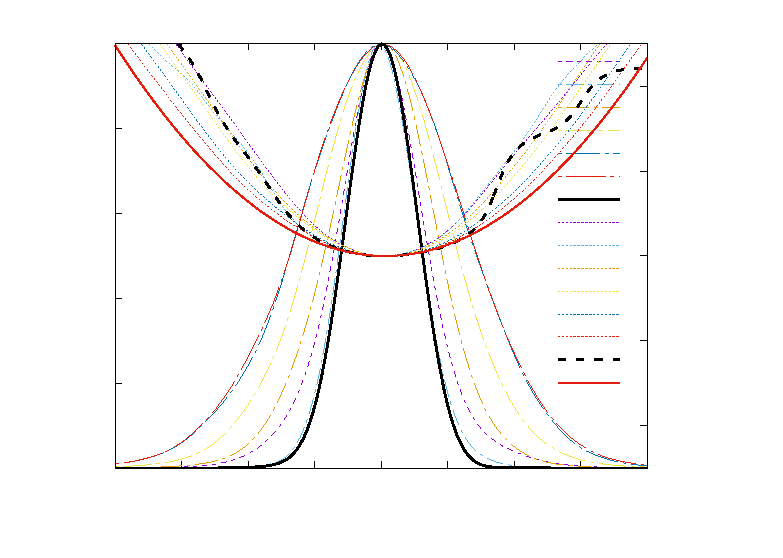
\includegraphics{temp1}}%
    \gplfronttext
  \end{picture}%
\endgroup

    \caption{blah}
    \label{fig:temp1}
\end{figure}
\begin{figure}[]
    \centering
    \input{spec1}
    \caption{blah}
    \label{fig:spec1}
\end{figure}
\begin{figure}[]
    \centering
    \input{temp2}
    \caption{blah2}
    \label{fig:temp2}
\end{figure}
\begin{figure}[]
    \centering
    % GNUPLOT: LaTeX picture with Postscript
\begingroup
  \makeatletter
  \providecommand\color[2][]{%
    \GenericError{(gnuplot) \space\space\space\@spaces}{%
      Package color not loaded in conjunction with
      terminal option `colourtext'%
    }{See the gnuplot documentation for explanation.%
    }{Either use 'blacktext' in gnuplot or load the package
      color.sty in LaTeX.}%
    \renewcommand\color[2][]{}%
  }%
  \providecommand\includegraphics[2][]{%
    \GenericError{(gnuplot) \space\space\space\@spaces}{%
      Package graphicx or graphics not loaded%
    }{See the gnuplot documentation for explanation.%
    }{The gnuplot epslatex terminal needs graphicx.sty or graphics.sty.}%
    \renewcommand\includegraphics[2][]{}%
  }%
  \providecommand\rotatebox[2]{#2}%
  \@ifundefined{ifGPcolor}{%
    \newif\ifGPcolor
    \GPcolortrue
  }{}%
  \@ifundefined{ifGPblacktext}{%
    \newif\ifGPblacktext
    \GPblacktexttrue
  }{}%
  % define a \g@addto@macro without @ in the name:
  \let\gplgaddtomacro\g@addto@macro
  % define empty templates for all commands taking text:
  \gdef\gplbacktext{}%
  \gdef\gplfronttext{}%
  \makeatother
  \ifGPblacktext
    % no textcolor at all
    \def\colorrgb#1{}%
    \def\colorgray#1{}%
  \else
    % gray or color?
    \ifGPcolor
      \def\colorrgb#1{\color[rgb]{#1}}%
      \def\colorgray#1{\color[gray]{#1}}%
      \expandafter\def\csname LTw\endcsname{\color{white}}%
      \expandafter\def\csname LTb\endcsname{\color{black}}%
      \expandafter\def\csname LTa\endcsname{\color{black}}%
      \expandafter\def\csname LT0\endcsname{\color[rgb]{1,0,0}}%
      \expandafter\def\csname LT1\endcsname{\color[rgb]{0,1,0}}%
      \expandafter\def\csname LT2\endcsname{\color[rgb]{0,0,1}}%
      \expandafter\def\csname LT3\endcsname{\color[rgb]{1,0,1}}%
      \expandafter\def\csname LT4\endcsname{\color[rgb]{0,1,1}}%
      \expandafter\def\csname LT5\endcsname{\color[rgb]{1,1,0}}%
      \expandafter\def\csname LT6\endcsname{\color[rgb]{0,0,0}}%
      \expandafter\def\csname LT7\endcsname{\color[rgb]{1,0.3,0}}%
      \expandafter\def\csname LT8\endcsname{\color[rgb]{0.5,0.5,0.5}}%
    \else
      % gray
      \def\colorrgb#1{\color{black}}%
      \def\colorgray#1{\color[gray]{#1}}%
      \expandafter\def\csname LTw\endcsname{\color{white}}%
      \expandafter\def\csname LTb\endcsname{\color{black}}%
      \expandafter\def\csname LTa\endcsname{\color{black}}%
      \expandafter\def\csname LT0\endcsname{\color{black}}%
      \expandafter\def\csname LT1\endcsname{\color{black}}%
      \expandafter\def\csname LT2\endcsname{\color{black}}%
      \expandafter\def\csname LT3\endcsname{\color{black}}%
      \expandafter\def\csname LT4\endcsname{\color{black}}%
      \expandafter\def\csname LT5\endcsname{\color{black}}%
      \expandafter\def\csname LT6\endcsname{\color{black}}%
      \expandafter\def\csname LT7\endcsname{\color{black}}%
      \expandafter\def\csname LT8\endcsname{\color{black}}%
    \fi
  \fi
    \setlength{\unitlength}{0.0500bp}%
    \ifx\gptboxheight\undefined%
      \newlength{\gptboxheight}%
      \newlength{\gptboxwidth}%
      \newsavebox{\gptboxtext}%
    \fi%
    \setlength{\fboxrule}{0.5pt}%
    \setlength{\fboxsep}{1pt}%
\begin{picture}(7200.00,5040.00)%
    \gplgaddtomacro\gplbacktext{%
      \csname LTb\endcsname%
      \put(814,704){\makebox(0,0)[r]{\strut{}$0$}}%
      \put(814,1518){\makebox(0,0)[r]{\strut{}$0.2$}}%
      \put(814,2332){\makebox(0,0)[r]{\strut{}$0.4$}}%
      \put(814,3147){\makebox(0,0)[r]{\strut{}$0.6$}}%
      \put(814,3961){\makebox(0,0)[r]{\strut{}$0.8$}}%
      \put(814,4775){\makebox(0,0)[r]{\strut{}$1$}}%
      \put(1457,484){\makebox(0,0){\strut{}$760$}}%
      \put(2479,484){\makebox(0,0){\strut{}$780$}}%
      \put(3501,484){\makebox(0,0){\strut{}$800$}}%
      \put(4522,484){\makebox(0,0){\strut{}$820$}}%
      \put(5544,484){\makebox(0,0){\strut{}$840$}}%
      \put(6187,1111){\makebox(0,0)[l]{\strut{}$-4$}}%
      \put(6187,1925){\makebox(0,0)[l]{\strut{}$-2$}}%
      \put(6187,2740){\makebox(0,0)[l]{\strut{}$0$}}%
      \put(6187,3554){\makebox(0,0)[l]{\strut{}$2$}}%
      \put(6187,4368){\makebox(0,0)[l]{\strut{}$4$}}%
    }%
    \gplgaddtomacro\gplfronttext{%
      \csname LTb\endcsname%
      \put(176,2739){\rotatebox{-270}{\makebox(0,0){\strut{}Spektrale Intensität $S$}}}%
      \put(6692,2739){\rotatebox{-270}{\makebox(0,0){\strut{}Phase $\Phi$ [rad]}}}%
      \put(3500,154){\makebox(0,0){\strut{}Wellenlänge $\lambda$ [nm]}}%
      \csname LTb\endcsname%
      \put(5068,4602){\makebox(0,0)[r]{\strut{}\tiny$S:0.95\;\text{nm}$}}%
      \csname LTb\endcsname%
      \put(5068,4382){\makebox(0,0)[r]{\strut{}\tiny$S:1.45\;\text{nm}$}}%
      \csname LTb\endcsname%
      \put(5068,4162){\makebox(0,0)[r]{\strut{}\tiny$S:1.95\;\text{nm}$}}%
      \csname LTb\endcsname%
      \put(5068,3942){\makebox(0,0)[r]{\strut{}\tiny$S:2.45\;\text{nm}$}}%
      \csname LTb\endcsname%
      \put(5068,3722){\makebox(0,0)[r]{\strut{}\tiny$S:2.84\;\text{nm}$}}%
      \csname LTb\endcsname%
      \put(5068,3502){\makebox(0,0)[r]{\strut{}\tiny$S:2.84\;\text{nm (opt)}$}}%
      \csname LTb\endcsname%
      \put(5068,3282){\makebox(0,0)[r]{\strut{}\tiny$\Phi:0.95\;\text{nm}$}}%
      \csname LTb\endcsname%
      \put(5068,3062){\makebox(0,0)[r]{\strut{}\tiny$\Phi:1.45\;\text{nm}$}}%
      \csname LTb\endcsname%
      \put(5068,2842){\makebox(0,0)[r]{\strut{}\tiny$\Phi:1.95\;\text{nm}$}}%
      \csname LTb\endcsname%
      \put(5068,2622){\makebox(0,0)[r]{\strut{}\tiny$\Phi:2.45\;\text{nm}$}}%
      \csname LTb\endcsname%
      \put(5068,2402){\makebox(0,0)[r]{\strut{}\tiny$\Phi:2.84\;\text{nm}$}}%
      \csname LTb\endcsname%
      \put(5068,2182){\makebox(0,0)[r]{\strut{}\tiny$\Phi:2.84\;\text{nm (opt)}$}}%
      \csname LTb\endcsname%
      \put(5068,1962){\makebox(0,0)[r]{\strut{}fit}}%
    }%
    \gplbacktext
    \put(0,0){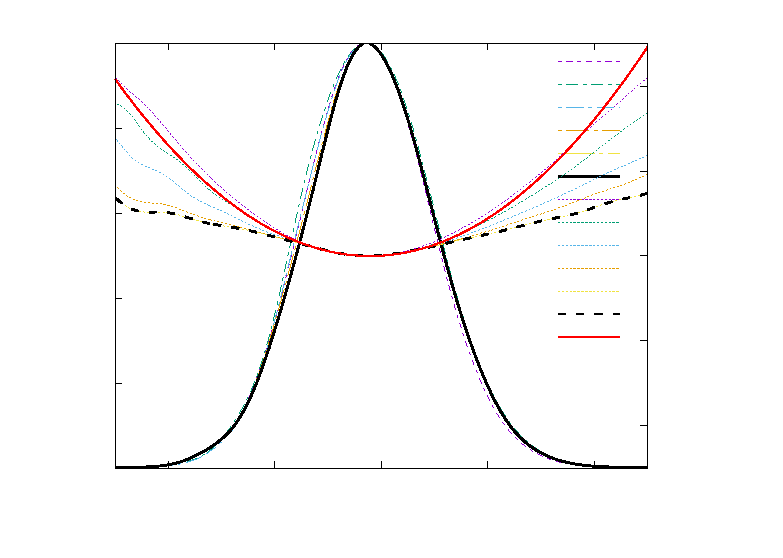
\includegraphics{spec2}}%
    \gplfronttext
  \end{picture}%
\endgroup

    \caption{blah2}
    \label{fig:spec2}
\end{figure}
\section{Diskussion}

\end{document}

